\documentclass[border=0pt]{standalone}

\usepackage{hyperref}
\usepackage{tikz}
\usepackage{graphicx}

\usetikzlibrary{decorations.pathreplacing,
  arrows,
  calc,
  decorations.pathmorphing,
  decorations.pathreplacing,
  decorations.markings,
  positioning,
  shapes
}
\tikzstyle{snakearrow} = [decorate, decoration={pre length=0.1cm,
  post length=0.1cm, snake, amplitude=.4mm,
  segment length=4mm},thick, ->]

\ifpdf
% Ensure reproducible output
\pdfinfoomitdate=1
\pdfsuppressptexinfo=-1
\pdftrailerid{}
\hypersetup{
  pdfcreator={},
  pdfproducer={}
}
\fi

\definecolor{pyorange}{rgb}{1.0,0.498,0.0549}
\definecolor{pyblue}{rgb}{0.122, 0.467, 0.706}

\begin{document}
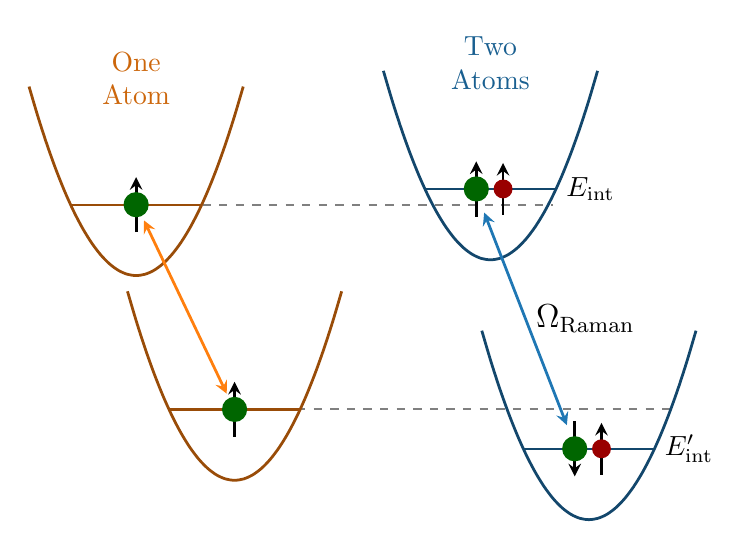
\begin{tikzpicture}
  \draw[gray, dashed, line width=0.7] (0, 0.9) -- ++(5.3, 0);
  \draw[gray, dashed, line width=0.7] (1.2, 0.9 - 2.6) -- ++(5.6, 0);

  \node[pyorange!80!black,align=center] at (0, 2.5) {One\\Atom};
  \draw[pyorange!60!black,line width=1]
  plot[domain={-0.8:0.8},smooth,variable=\x] ({\x * 1.7}, {(\x)^2 * 3.75});
  \draw[pyorange!60!black,line width=0.8] ({-sqrt(0.9 / 3.75) * 1.7}, 0.9) --
  coordinate (Unshift1) ({sqrt(0.9 / 3.75) * 1.7}, 0.9);
  \draw[->,>=stealth,line width=1] ($(Unshift1) - (0, 0.35)$) -- ($(Unshift1) + (0, 0.35)$);
  \fill[green!40!black] (Unshift1) circle (0.16);

  \draw[pyorange!60!black,line width=1]
  plot[domain={-0.8:0.8},smooth,variable=\x] ({\x * 1.7 + 1.25}, {(\x)^2 * 3.75 - 2.6});
  \draw[pyorange!60!black,line width=0.8] ({-sqrt(0.9 / 3.75) * 1.7 + 1.25}, 0.9 - 2.6) --
  coordinate (Unshift2) ({sqrt(0.9 / 3.75) * 1.7 + 1.25}, 0.9 - 2.6);
  \draw[->,>=stealth,line width=1] ($(Unshift2) - (0, 0.35)$) -- ($(Unshift2) + (0, 0.35)$);
  \fill[green!40!black] (Unshift2) circle (0.16);

  \draw[<->,>=stealth,line width=1,pyorange]
  ($(Unshift1) + (0.1, -0.2)$) -- ($(Unshift2) - (0.1, -0.2)$);

  \begin{scope}[shift={(4.5, 0)}]
    \begin{scope}[shift={(0, 0.2)}]
      \node[pyblue!80!black,align=center] at (0, 2.5) {Two\\Atoms};
      \draw[pyblue!60!black,line width=1]
      plot[domain={-0.8:0.8},smooth,variable=\x] ({\x * 1.7}, {(\x)^2 * 3.75});
      \draw[pyblue!60!black,line width=0.8] ({-sqrt(0.9 / 3.75) * 1.7}, 0.9) --
      coordinate (Shift1) ({sqrt(0.9 / 3.75) * 1.7}, 0.9) node[black,right] {$E_{\mathrm{int}}$};
      \draw[->,>=stealth,line width=1] ($(Shift1) + (-0.18, -0.35)$)
      -- ($(Shift1) + (-0.18, 0.35)$);
      \fill[green!40!black] ($(Shift1) + (-0.18, 0)$) circle (0.16);
      \draw[->,>=stealth,line width=1] ($(Shift1) + (0.16, -0.33)$)
      -- ($(Shift1) + (0.16, 0.33)$);
      \fill[red!60!black] ($(Shift1) + (0.16, 0)$) circle (0.12);
    \end{scope}

    \begin{scope}[shift={(0, -0.5)}]
      \draw[pyblue!60!black,line width=1]
      plot[domain={-0.8:0.8},smooth,variable=\x] ({\x * 1.7 + 1.25}, {(\x)^2 * 3.75 - 2.6});
      \draw[pyblue!60!black,line width=0.8] ({-sqrt(0.9 / 3.75) * 1.7 + 1.25}, 0.9 - 2.6) --
      coordinate (Shift2) ({sqrt(0.9 / 3.75) * 1.7 + 1.25}, 0.9 - 2.6)
      node[black,right] {$E_{\mathrm{int}}'$};
      \draw[<-,>=stealth,line width=1] ($(Shift2) + (-0.18, -0.35)$)
      -- ($(Shift2) + (-0.18, 0.35)$);
      \fill[green!40!black] ($(Shift2) + (-0.18, 0)$) circle (0.16);
      \draw[->,>=stealth,line width=1] ($(Shift2) + (0.16, -0.33)$)
      -- ($(Shift2) + (0.16, 0.33)$);
      \fill[red!60!black] ($(Shift2) + (0.16, 0)$) circle (0.12);
    \end{scope}
    \draw[<->,>=stealth,line width=1,pyblue]
    ($(Shift1) + (-0.08, -0.3)$) --
    node[black,right] {\large $\Omega_{\mathrm{Raman}}$}
    ($(Shift2) + (-0.28, 0.3)$);
  \end{scope}
\end{tikzpicture}
\end{document}
